\documentclass{article}

% Language setting
% Replace `english' with e.g. `spanish' to change the document language
\usepackage[english]{babel}
\usepackage{float} % Add this package
% Set page size and margins
% Replace `letterpaper' with `a4paper' for UK/EU standard size
\usepackage[letterpaper,top=2cm,bottom=2cm,left=3cm,right=3cm,marginparwidth=1.75cm]{geometry}
\usepackage{xcolor}
% Define colors for syntax highlighting
\definecolor{codegreen}{rgb}{0,0.6,0}   % Green for comments
\definecolor{codegray}{rgb}{0.5,0.5,0.5} % Gray for line numbers
\definecolor{codepurple}{rgb}{0.58,0,0.82} % Purple for strings
\definecolor{backcolour}{rgb}{1,1,1}    % White background
\usepackage{amsthm}

% Define a new "exercise" environment with numbering
\newtheorem{exercise}{Exercise}[section]
\usepackage{listings}
\usepackage{tikz}

% Configure listings
\lstset{
    backgroundcolor=\color{backcolour}, % White background
    commentstyle=\color{codegreen},     % Green comments
    keywordstyle=\color{magenta},       % Magenta keywords
    numberstyle=\tiny\color{codegray},  % Gray line numbers
    stringstyle=\color{codepurple},     % Purple strings
    basicstyle=\ttfamily\footnotesize,  % Monospace font
    breakatwhitespace=false,            % No breaks at whitespace
    breaklines=true,                    % Break long lines
    captionpos=b,                       % Caption at bottom
    keepspaces=true,                    % Keep spaces
    numbers=left,                       % Line numbers on left
    numbersep=5pt,                      % Distance of line numbers from code
    showspaces=false,                   % Don't show spaces
    showstringspaces=false,             % Don't show spaces in strings
    showtabs=false,                     % Don't show tabs
    tabsize=2,                          % Tab size
    frame=single,                       % Frame around the listing
    rulecolor=\color{black},            % Frame color
    escapeinside={\%*}{*)},             % Escape to LaTeX
    xleftmargin=20pt,                   % Left margin
    framexleftmargin=20pt,              % Frame left margin
}

% Useful packages
\usepackage{amsmath}
\usepackage{graphicx}
\usepackage[colorlinks=true, allcolors=blue]{hyperref}

\title{CP Search exercises}
\author{Pierre Schaus, UCLouvain, ICTEAM}

\begin{document}
    \maketitle

    \begin{abstract}
    This document contains exercises related to the search topic in constraint programming.
    Those exercises are proposed in the ACP summer school on constraint programming at Benin.
    \end{abstract}

    \section{TinyCSP has lost its search}

    In this exercise, we will study a simple CSP solver in Java called TinyCSP.
    Let us first see how to model the NQueens problem using TinyCSP.
    The NQueens problem is to place N queens on an N x N chessboard such that no two queens threaten each other.
    The model is given in the code Listing~\ref{nqueen} below.

    \begin{minipage}{\linewidth}
        \lstinputlisting[language=Java, label=nqueen, caption={NQueens Model using TinyCSP}, escapeinside={(*@}{@*)}]{figures/NQueens.java}
    \end{minipage}

    The domain to represent the values of the variables is implemented in the class \texttt{Domain} and the variables are instances of the class \texttt{Domain}.
    It is a simple implementation of a domain using a \texttt{BitSet} to represent the set of values in the domain.


    \begin{minipage}{\linewidth}
        \lstinputlisting[language=Java,caption={Domain Implementation in TinyCSP}, escapeinside={(*@}{@*)}]{figures/Domain.java}
    \end{minipage}



    The Variable implementatino is very simple, it just contains a domain.

    \begin{minipage}{\linewidth}
        \lstinputlisting[language=Java,caption={Variable Implementation in TinyCSP}, escapeinside={(*@}{@*)}]{figures/Variable.java}
    \end{minipage}


    Constraint is an abstract class with an absract method \texttt{propagate()}
    that is called by the solver to remove inconsistent values from the domains of the variables involved in the constraint.
    It also returns true if any value could be removed from the domains of the variables involved in the constraint.
    The constraint can also throw an \texttt{Inconsistency} exception if the constraint is not satisfiable.

    In TinyCSP, we have only one constraint implemented, the \texttt{NotEqual} constraint.
    Of course feel free to implement more constraints during your free times.

    \begin{minipage}{\linewidth}
        \lstinputlisting[language=Java,caption={Constraints Implementation in TinyCSP}, escapeinside={(*@}{@*)}]{figures/Constraint.java}
    \end{minipage}


    The TinyCSP solver class is the main class that implements the solver.
    It contains a list of constraints and a list of variables.
    The solver provides factory methods to create variables, add constraints, and trigger fix point propagation.
    Unfortunately, the search is not implemented yet.

    \begin{exercise}
        Your task is to implement the depth search algorithm.
        If you need some hint, you can look at the Listing~\ref{shuffled_dfs} below
        that contains the shuffled lines of code to complete the \texttt{dfsNary} method.
    \end{exercise}

    \begin{minipage}{\linewidth}
        \lstinputlisting[language=Java, label=tinycsp, caption={TinyCSP Solver class}, escapeinside={(*@}{@*)}]{figures/TinyCSP.java}
    \end{minipage}

    \begin{minipage}{\linewidth}
        \lstinputlisting[language=Java, label=shuffled_dfs, caption={Shuffled lines for completing the dfsNary of Listing~\ref{tinycsp}},escapeinside={(*@}{@*)}]{figures/DFSShuffle.java}
    \end{minipage}

    As you might have noticed the variable selection is very simple,
    it just selects the first variable that is not fixed.
    Now that you are convinced about the importance of the first fail heuristic,
    let us implement it in the next exercise.

    \begin{exercise}
        Your task is to implement the first fail heuristic in Listing~\ref{ff}.
        To help you, we have provided the shuffled lines of code in Listing~\ref{shuffled_ff} below.
        Of course, don't forget to adapt your code for the search algorithm
        in Listing~\ref{tinycsp} to call your new first fail heuristic.
    \end{exercise}

    \begin{minipage}{\linewidth}
        \lstinputlisting[language=Java, label=ff, caption={First fail},escapeinside={(*@}{@*)}]{figures/FirstFail.java}
    \end{minipage}

    \begin{minipage}{\linewidth}
        \lstinputlisting[language=Java, label=shuffled_ff, caption={Suffled lines for completing the first fail of Listing~\ref{ff}},escapeinside={(*@}{@*)}]{figures/FirstFailShuffle.java}
    \end{minipage}


    \section{Backtracking Search with Sparse-Sets}



    \section{Black-Box Search for Variable Heuristics}



    \begin{exercise}
        Consider seven variables $X, Y, Z, A, B, C, D$ such that:

        \begin{itemize}
        \item $X, Y, Z$ have the domain $\{0,1\}$ and there are no constraints on these variables.
        \item $A, B, C, D$ have the domain $\{0,1,2\}$ and there is a single constraint: $AllDifferent(A, B, C, D)$ implemented using forward checking (only fixed variables are removed from the domains of the other unfixed variables).
        \end{itemize}
        Consider a \emph{conflict-ordering search} that, by default,
        considers the variables in the order given above $X \leftarrow  Y \leftarrow  Z \leftarrow  A \leftarrow  B \ldots $ and always tries,
        given a selected variable $V$, $V = V.min()$ on the left branch, and $V \neq V.min()$ on the right branch.

        There are no solutions to this problem.
        Draw the search tree.
        How many nodes will be visited by the solver?
    \end{exercise}

    \section{Value Heuristics}

    \section{Discrepancy Search}

    \begin{exercise}
        A complete binary tree of depth 4 was pruned by a limited discrepancy search.
        The resulting tree is shown in Figure~\ref{fig:discrepancy1}.
        What do you tink was the dicrepancy limit used to prune the tree?
        \label{ex:discrepancy1}
    \end{exercise}

    \begin{figure}[htbp]
        \centering
        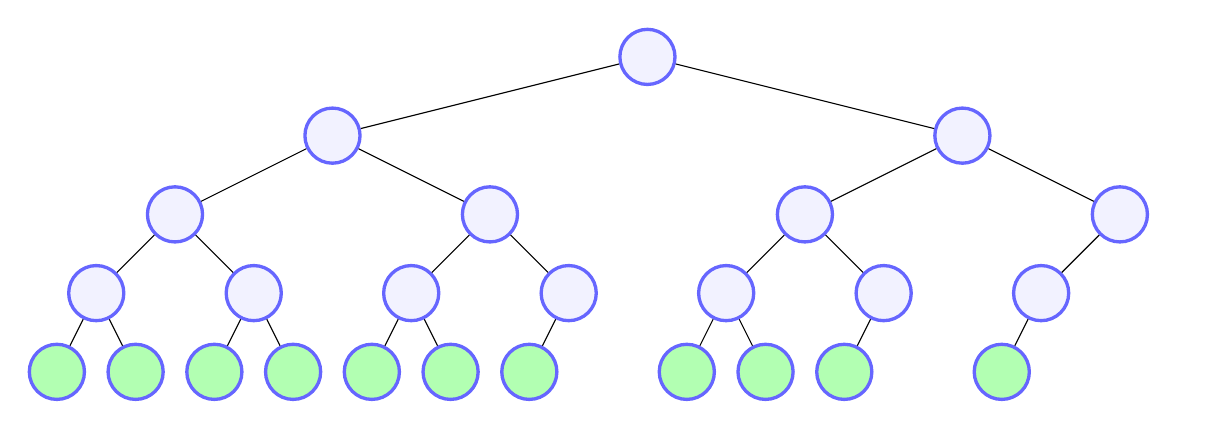
\begin{tikzpicture}[
    level distance=1cm,
    level 1/.style={sibling distance=8cm},
    level 2/.style={sibling distance=4cm},
    level 3/.style={sibling distance=2cm},
    level 4/.style={sibling distance=1cm},
    level 5/.style={sibling distance=0.5cm},
    every node/.style={circle, draw=blue!60, fill=blue!5, very thick, minimum size=7mm},
    phantom/.style={coordinate},
    invisible/.style={edge from parent/.style={draw=none}}
]

% Root node
    \node {}
    % --- Left branch (0 discrepancy)
    child {
        node {}
        % --- LL (still 0 discrepancy)
        child {
            node {}
            % --- LLL (still 0 discrepancy)
            child {
                node {}
                child { node[fill=green!30] {} } % depth 5 leaf
                child { node[fill=green!30] {} } % depth 5 leaf
            }
            % --- LLR (1 discrepancy)
            child {
                node {}
                child { node[fill=green!30] {} }
                child { node[fill=green!30] {} }
            }
        }
        % --- LR (1 discrepancy)
        child {
            node {}
            % --- LRL (1 discrepancy)
            child {
                node {}
                child { node[fill=green!30] {} }
                child { node[fill=green!30] {} }
            }
            % --- LRR (2 discrepancies, allowed but stop deeper rights)
            child {
                node {}
                child { node[fill=green!30] {} }
                child[phantom, invisible]
            }
        }
    }
    % --- Right branch (1 discrepancy)
    child {
        node {}
        % --- RL (1 discrepancy)
        child {
            node {}
            % --- RLL (1 discrepancy)
            child {
                node {}
                child { node[fill=green!30] {} }
                child { node[fill=green!30] {} }
            }
            % --- RLR (2 discrepancies, allowed but stop deeper rights)
            child {
                node {}
                child { node[fill=green!30] {} }
                child[phantom, invisible]
            }
        }
        % --- RR (2 discrepancies, allowed but no further rights)
        child {
            node {}
            % --- RRL (2 discrepancies)
            child {
                node {}
                child { node[fill=green!30] {} }
                child[phantom, invisible]
            }
            % --- RRR (would be 3 discrepancies → prune)
            child[phantom, invisible]
        }
    };
\end{tikzpicture}
        \caption{Exercise~\ref{ex:discrepancy1}.}
        \label{fig:discrepancy1}
    \end{figure}

    \begin{exercise}
        Consider binary tree shown in Figure~\ref{fig:discrepancy2}.
        What is the lowest discrepancy limit that could be used to that no nodes are pruned?
        \label{ex:discrepancy2}
    \end{exercise}

    \begin{exercise}
        Color the nodes in red in Figure~\ref{fig:discrepancy2} corresponding to the nodes that would be pruned by
        a limited discrepancy search with a discrepancy limit of 2.
        \label{ex:discrepancy3}
    \end{exercise}

    \begin{figure}[htbp]
        \centering
        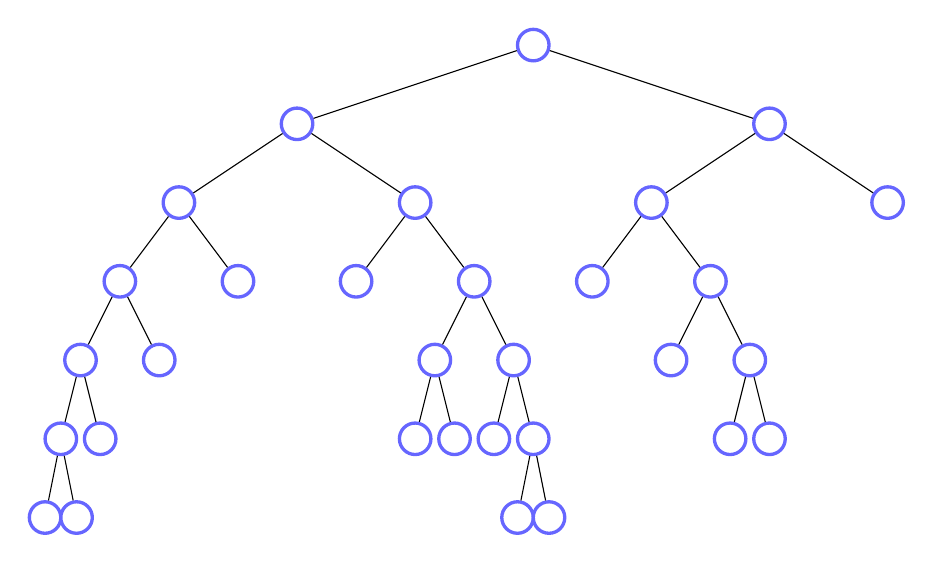
\begin{tikzpicture}[
    level distance=1cm,
    level 1/.style={sibling distance=6cm},
    level 2/.style={sibling distance=3cm},
    level 3/.style={sibling distance=1.5cm},
    level 4/.style={sibling distance=1cm},
    level 5/.style={sibling distance=0.5cm},
    level 6/.style={sibling distance=0.4cm},
    every node/.style={circle, draw=blue!60, fill=white, very thick, minimum size=4mm},
    phantom/.style={coordinate},
    invisible/.style={edge from parent/.style={draw=none}}
]

% Root node
    \node {}
    child {
        node {} % left child depth 1
        child {
            node {} % left-left depth 2
            child {
                node {} % left-left-left depth 3
                child {
                    node {} % depth 4
                    child { node {}
                        child { node {} }
                        child { node {} }% leaf depth 5
                    } % leaf depth 5
                    child { node {} } % leaf depth 5
                }
                child { node {} } % leaf depth 4
            }
            child { node {} } % leaf depth 3
        }
        child {
            node {} % left-right depth 2
            child { node {} } % leaf depth 3
            child {
                node {} % depth 3
                child {
                    node {} % depth 4
                    child { node {} } % leaf depth 5
                    child { node {} } % leaf depth 5
                }
                child {
                    node {} % depth 4
                    child { node {} } % leaf depth 5
                    child {
                        node {} % depth 5
                        child { node {} } % leaf depth 6
                        child { node {} } % leaf depth 6
                    }
                }
            }
        }
    }
    child {
        node {} % right child depth 1
        child {
            node {} % right-left depth 2
            child { node {} } % leaf depth 3
            child {
                node {} % depth 3
                child { node {} } % leaf depth 4
                child {
                    node {} % depth 4
                    child { node {} } % leaf depth 5
                    child {
                        node {} % depth 5
                    }
                }
            }
        }
        child { node {} } % leaf depth 2
    };
\end{tikzpicture}
        \caption{Exercise~\ref{ex:discrepancy2} and~\ref{ex:discrepancy3}.}
        \label{fig:discrepancy2}
    \end{figure}

    \section{Breaking Symmetries}

    \subsection{With constraints ...}

    Consider a graph with 6 vertices arranged in a hexagon (each vertex connected to its two immediate neighbors).
    The goal is to color each vertex with one of 3 colors (e.g., Red, Green, Blue) such that no two adjacent vertices share the same color.

    \begin{figure}[htbp]
        \centering
        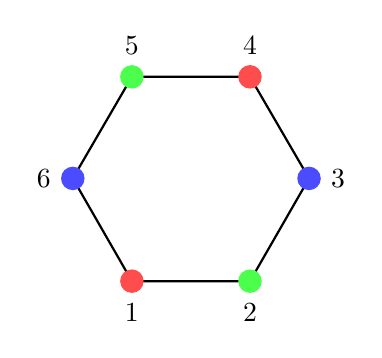
\begin{tikzpicture}[scale=1.5]
  % Define colors
  \colorlet{red}{red!70}
  \colorlet{green}{green!70}
  \colorlet{blue}{blue!70}

  % Draw the hexagon
  \draw[thick] (0,0) -- (1,0) -- (1.5,0.87) -- (1,1.73) -- (0,1.73) -- (-0.5,0.87) -- cycle;

  % Label and color the vertices
  \node[fill=red, circle, inner sep=3pt, label=below:1] at (0,0) {};
  \node[fill=green, circle, inner sep=3pt, label=below:2] at (1,0) {};
  \node[fill=blue, circle, inner sep=3pt, label=right:3] at (1.5,0.87) {};
  \node[fill=red, circle, inner sep=3pt, label=above:4] at (1,1.73) {};
  \node[fill=green, circle, inner sep=3pt, label=above:5] at (0,1.73) {};
  \node[fill=blue, circle, inner sep=3pt, label=left:6] at (-0.5,0.87) {};

\end{tikzpicture}
        \caption{Exercise~\ref{ex:symmetry1}.}
        \label{fig:symmetry1}
    \end{figure}

    \begin{exercise}
        Propose a CSP model for the hexagon problem (variables, domains, constraints).
        \begin{verbatim}
            ....
            ....
            ...
        \end{verbatim}
        \label{ex:symmetry1}
    \end{exercise}


    \begin{exercise}
        List 3 type of symmetries in the hexagon problem.
        \label{ex:symmetry2}
    \end{exercise}

    \begin{exercise}
        Given a solution to the hexagon problem, how many symmetric solutions can you generate
        using each type of symmetry ?
        \label{ex:symmetry3}
    \end{exercise}

    \begin{exercise}
        Given a solution to the hexagon problem,
        propose a symmetry breaking constraint that can be used to eliminate symmetric solutions.
        \label{ex:symmetry4}
    \end{exercise}


    \begin{exercise}
        We consider an alternative model for the n-queens problem, where the n-variables $q_1 \ldots,q_n$
        correspond to the $n$ queens and the domain of each variable
        is the set of integers $\{1,2,\ldots,n^2\}$, representing the squares on the chessboard.
        Thus an assignment $q_i=a$ means that the $i$th queen is on square $a$.
        Which statements are valid regarding the symmetries of this model?
        \begin{itemize}
            \item This model presents more symmetries than the classical n-queens formulation with one variable per column and the domain representing the row.
            \item This model presents less symmetries than the classical n-queens formulation with one variable per column and the domain representing the row.
            \item Since I can create a mapping between the variables preserving the (non)-solution, this model presents variable symmetries
        \end{itemize}
        \label{ex:queens_symmetry1}
    \end{exercise}

    \begin{exercise}
        Considering the alternative model for the n-queens problem from Exercise~\ref{ex:queens_symmetry1},
        Assume that we use search heuristic denoted by $H$, and we break the symmetries by adding the constraints
        $q_1<q_2< \ldots <q_n$ to our model.
        Which statements are valid?
        \begin{itemize}
            \item The number of backtracks required using heuristic $H$ to find the first solution might be larger or smaller, but hopefully smaller
            \item The number of solutions output by my model when enumerating them all is reduced by a factor $n!$ (factorial)
            \item The number of backtracks required using heuristic $H$ to find the first solution is always reduced since the search tree to explore is smaller.
        \end{itemize}
        \label{ex:queens_symmetry2}
    \end{exercise}

    \subsection{With the search ...}

    The bin-packing problem is to pack a set of items into a number of bins while satisfying the capacity of the bins.
    This problem can be modeled as a CSP using one variable per item, each with a domain representing the bin in which the item is packed.


    \begin{exercise}
        Consider a bin-packing problem with the items of weights $[1,2,2,2,3,3,4,4]$ and 4 empty bins of capacity 6.
        In a node of the search tree, we have the following partial assignment.
        $X_0=0,X_4=0,X_1=1,X_2=1$.
        \begin{itemize}
            \item  Represent the item placed in each bin corresponding to the assignment in Figure~\ref{fig:symmetry2}.
            \item  The variable $X_5$ is the next unassigned variable selected by the search heuristic. What are the possible values for $X_5$? What branches must then be considered for avoiding the exploration of symmetric solutions?
        \end{itemize}
        \label{symmetry2}
    \end{exercise}

    \begin{figure}[htbp]
        \centering
        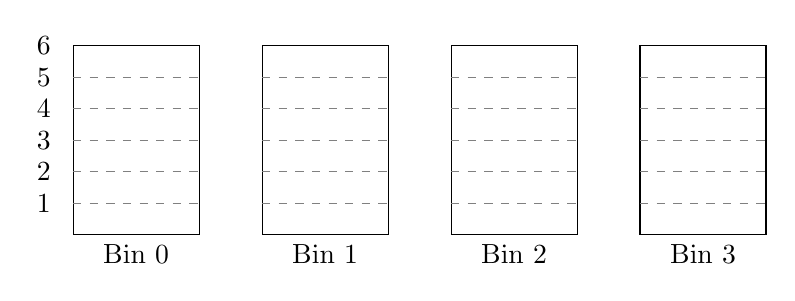
\begin{tikzpicture}[scale=0.8, bin/.style={minimum width=2cm, minimum height=0.5cm, draw, anchor=south west}]

    % Bin 0
    \draw (0,0) rectangle (2,3);
    \foreach \y in {0.5,1.0,1.5,2.0,2.5} {
        \draw[dashed, gray] (0,\y) -- (2,\y);
    }
    \node at (1, -0.3) {Bin 0};

    % Bin 1
    \draw (3,0) rectangle (5,3);
    \foreach \y in {0.5,1.0,1.5,2.0,2.5} {
        \draw[dashed, gray] (3,\y) -- (5,\y);
    }
    \node at (4, -0.3) {Bin 1};

    % Bin 2
    \draw (6,0) rectangle (8,3);
    \foreach \y in {0.5,1.0,1.5,2.0,2.5} {
        \draw[dashed, gray] (6,\y) -- (8,\y);
    }
    \node at (7, -0.3) {Bin 2};

    % Bin 3
    \draw (9,0) rectangle (11,3);
    \foreach \y in {0.5,1.0,1.5,2.0,2.5} {
        \draw[dashed, gray] (9,\y) -- (11,\y);
    }
    \node at (10, -0.3) {Bin 3};

    % Y-axis labels for capacity (optional)
    \foreach \y/\label in {0.5/1,1.0/2,1.5/3,2.0/4,2.5/5} {
        \node[left] at (-0.2,\y) {\label};
    }
    \node[left] at (-0.2,3) {6};
\end{tikzpicture}
        \caption{Exercise~\ref{ex:symmetry2}.}
        \label{fig:symmetry2}
    \end{figure}



    \section{Large Neighborhood Search}
    
    \begin{exercise}
        For modeling the traveling salesman problem (TSP) using CP, one can use a successor array representation.
        The variable $X_i$ represents the city visited after city $i$.
        Then one need one $\texttt{circuit}X_1 \ldots X_n)$ global constraint to ensure that the tour is a single cycle.
        For the circuit on the left of Figure~\ref{fig:lns1} and the successor array representation,
        give the assignment to the variables:
        \begin{equation*}
            X_0 = \ldots, X_1 = \ldots, X_2 = \ldots, X_3 = \ldots,X_4 = \ldots, X_5 = \ldots, X_6 = \ldots.
        \end{equation*}
        \label{ex:lns1}
    \end{exercise}


    \begin{figure}[htbp]
        \centering
        \includegraphics[scale=0.5]{figures/lns1.pdf}
        \caption{Exercise~\ref{ex:lns1}.}
        \label{fig:lns1}
    \end{figure}

    \section{Restarts}

    \bibliographystyle{alpha}
    \bibliography{biblio}
\end{document}
